\documentclass[xcolor={dvipsnames}, handout]{beamer}
%\documentclass[xcolor={dvipsnames}]{beamer}
%\usepackage{amsmath,amsfonts,amssymb,pxfonts,eulervm,xspace}
\usepackage{amsmath, amsfonts, amssymb, mathtools, eulervm, xspace}
\renewcommand{\restriction}{\mathord{\upharpoonright}} %restriction w/p space
\usepackage{bm}
\usepackage{mathrsfs} % math script fonts
\usepackage{tikz}
\usetikzlibrary{cd} % commutative diagrams
\newtheorem{prop}{Proposition} %math?

\usepackage{subcaption} % subfigure float captioning

\usepackage{tabulary}
\usepackage{tabularx}
\usepackage{booktabs}
\usepackage{multirow}
\usepackage{array}

\usepackage{graphicx}
\usepackage{adjustbox}%scale tikz-cd

\usepackage{appendixnumberbeamer} 
\usepackage{comment}
\usepackage{minted}
\setminted[python]{fontsize=\scriptsize, 
                   linenos,
                   numbersep=8pt,
                   autogobble, 
                   frame=lines,
                   bgcolor=bg,
                   framesep=3mm} 
\usepackage{notation} % move this later

\graphicspath{.figures/}

\usepackage[backend=bibtex, sorting=none, doi=false,isbn=false,url=false, giveninits=true]{biblatex}
\bibliographystyle{plain}
\bibliography{../paper/bibliography.bib}

%\usetheme{ccnycrest}

\newenvironment{changemargin}[2]{%
\begin{list}{}{%
\setlength{\topsep}{0pt}%
\setlength{\leftmargin}{#1}%
\setlength{\rightmargin}{#2}%
\setlength{\listparindent}{\parindent}%
\setlength{\itemindent}{\parindent}%
\setleng{}th{\parsep}{\parskip}%
}%
\item[]}{\end{list}}

\begin{document}

\title{Topological Equivariant Artist Model}
\begin{comment}
\begin{frame}
	\titlepage
    Hannah Aizenman, Tom Caswell, Michael Grossberg\\
    %Committee: Dr. Robert Haralick, Dr. Lev Manovich, Dr. Huy Vo\\
    %External Member: Dr. Marcus Hanwell
\end{frame}

\section{Introduction}
\begin{frame}{What are we doing?}
    \begin{itemize}
        \item develop a model for describing data to graphic transformations
        \item specify a visualization library architecture based on this model
        \item implement functional(ish) components based on this model using ideas from functional programming
    \end{itemize}
\end{frame}

%% maybe pull out the middle for now? move the 3 stages down to construction? 
\begin{frame}{What do visualization libraries do?}
    \begin{figure}
        \begin{overprint}
            \onslide<1|handout:1>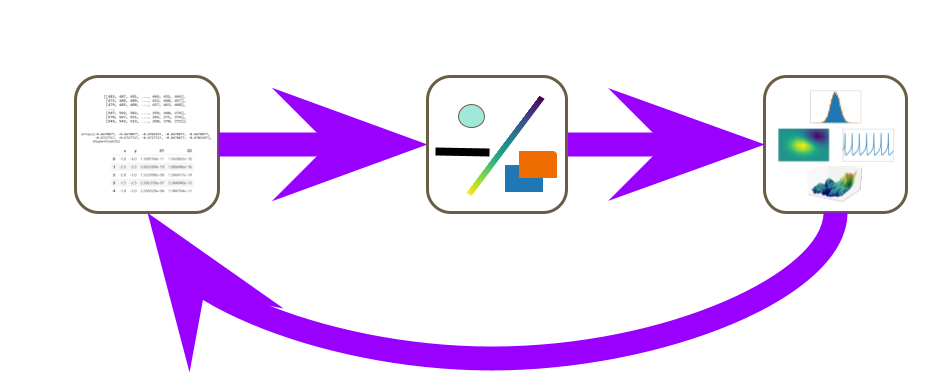
\includegraphics[width=\linewidth]{figures/flow/s2.png}
            \onslide<2|handout:2>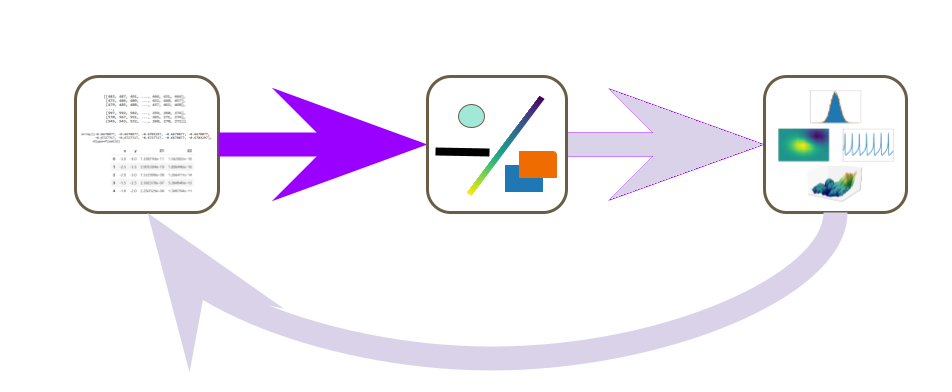
\includegraphics[width=\linewidth]{figures/flow/s_vc.png}
            \onslide<3|handout:3>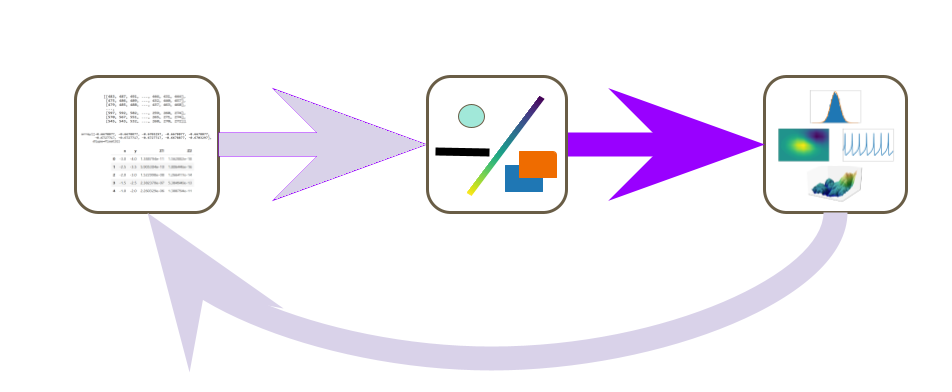
\includegraphics[width=\linewidth]{figures/flow/s_mark.png}
            \onslide<4|handout:4>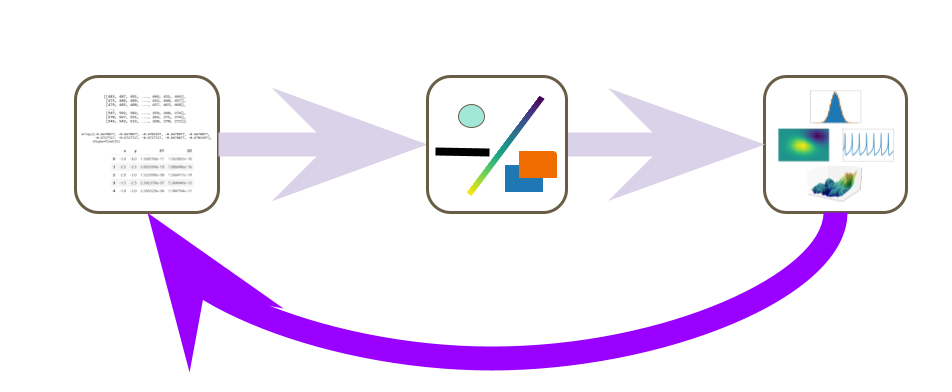
\includegraphics[width=\linewidth]{figures/flow/s3.png}
        \end{overprint}
    \end{figure}
\end{frame}

\begin{frame}{Case Study: Matplotlib}
    \begin{figure}
       
\includegraphics[width=\linewidth]{figures/flow/artists.png}
    \end{figure}
\end{frame}

\begin{frame}{Visualizations Preserve Structure}
    \begin{description}
        \item [continuity] topological properties \cite{wilkinsonGrammarGraphics2005}, i.e. how elements in a dataset are organized, e.g. discrete rows in a table, networked nodes, pixels in an image, points on a line
        \item [equivariance] data and visual encodings are matched such that transformations have an equivalent effect on data and graphical representations, e.g. rotating a matrix and image, shifting  points on a line and a line graphic
      \end{description}
\end{frame}

\begin{frame}{Continuity}
    \begin{figure}
        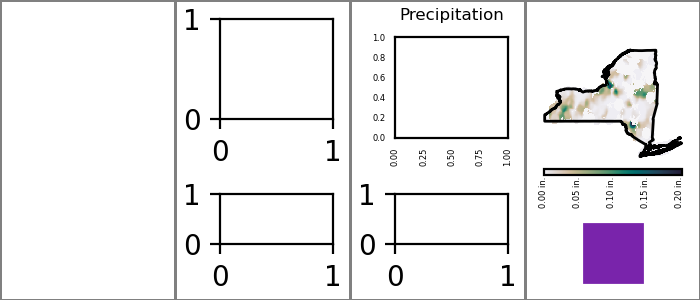
\includegraphics[width=\linewidth]{../paper/figures/k_different_types.png}
    \end{figure}
\end{frame}

\begin{frame}{Expressed in container}    
    \begin{figure}
        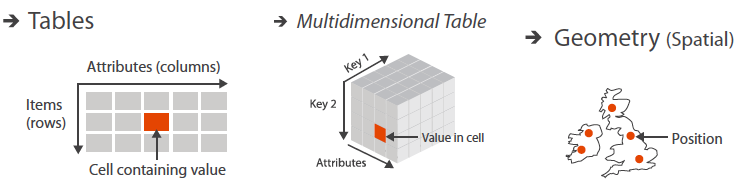
\includegraphics[width=1\textwidth]{figures/intro/munzner_datatypes.png}
        \caption{Figure 2.8 in Munzner's Visualization Analysis and Design\cite{munznerVisualizationAnalysisDesign2014}}
    \end{figure}
\end{frame}

\begin{frame}{Why is container type not enough?}
    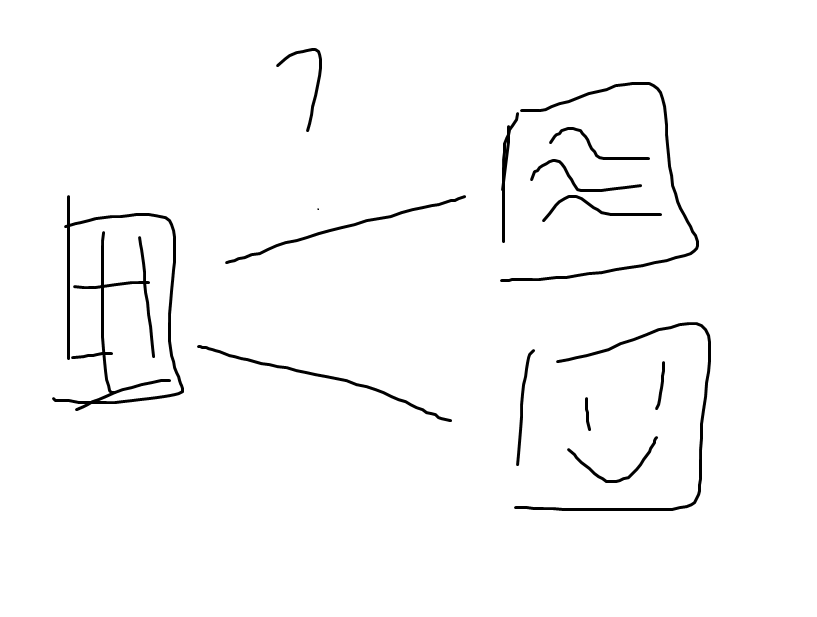
\includegraphics[width=1\linewidth]{../paper/figures/whycontinuity.png}
\end{frame}

\begin{frame}{Equivariance}
    \begin{description}
        \item[Retinal Variables \& Marks] visual encodings should match properties of the data \cite{bertinSemiologyGraphicsDiagrams2011a}
        \pause
        \item[Graphical Integrity] graphs show \textbf{only} the data\cite{tufteVisualDisplayQuantitative2001}
        \pause 
        \item[Naturalness] easier to understand when properties match\cite{norman_things_smart}
        \pause
        \item[Expressiveness] which structure preserving mappings can a tool implement\cite{mackinlayAutomatingDesignGraphical1986}] 
    \end{description}
\end{frame}

%flip columns
\begin{frame}{Frameworks for Expressing Visual Equivariance}
    \begin{description}
        \item[linguistically] visualization has syntax, semantics, grammar expresses how to design structure preserving visualizations
        \cite{mackinlayAutomatingDesignGraphical1986,mackinlayAUTOMATICDESIGNGRAPHICAL1987,wilkinsonGrammarGraphics2005}

        \item[algebraically] transformations on data and graphics are equivalent symmetric \cite{kindlmannAlgebraicProcessVisualization2014}
        \begin{columns}
            \column{.5\textwidth}
            \begin{description}
                \item[D] data 
                \item[R] data representation 
                \item[V] visualization
            \end{description}
            \column{.5\textwidth}
            \begin{equation*}
                \begin{tikzcd}[ampersand replacement=\&]
                    D \arrow[d, "\alpha"'] \arrow[r, "r_1"] \& R \arrow[r, "\nu"]  \& V \arrow[d, "\omega"] \\
                    D \arrow[r, "r_2"']                     \& R \arrow[r, "\nu"'] \& V                    
                \end{tikzcd}
                \end{equation*}
        \end{columns} 
    \item[categorically] \textit{understanding} = \textit{read} $\circ$ \textit{render} \cite{vickersUnderstandingVisualizationFormal2013}    
    \end{description}
\end{frame}

\begin{frame}{Domain specific libraries know their structure\cite{HeerSoftware2006}}
    \begin{table}
        %\renewcommand{\arraystretch}{2}
        %
        \begin{tabular}{>{\onslide<1->}l>{\onslide<2->}l>{\onslide<3->}l}
            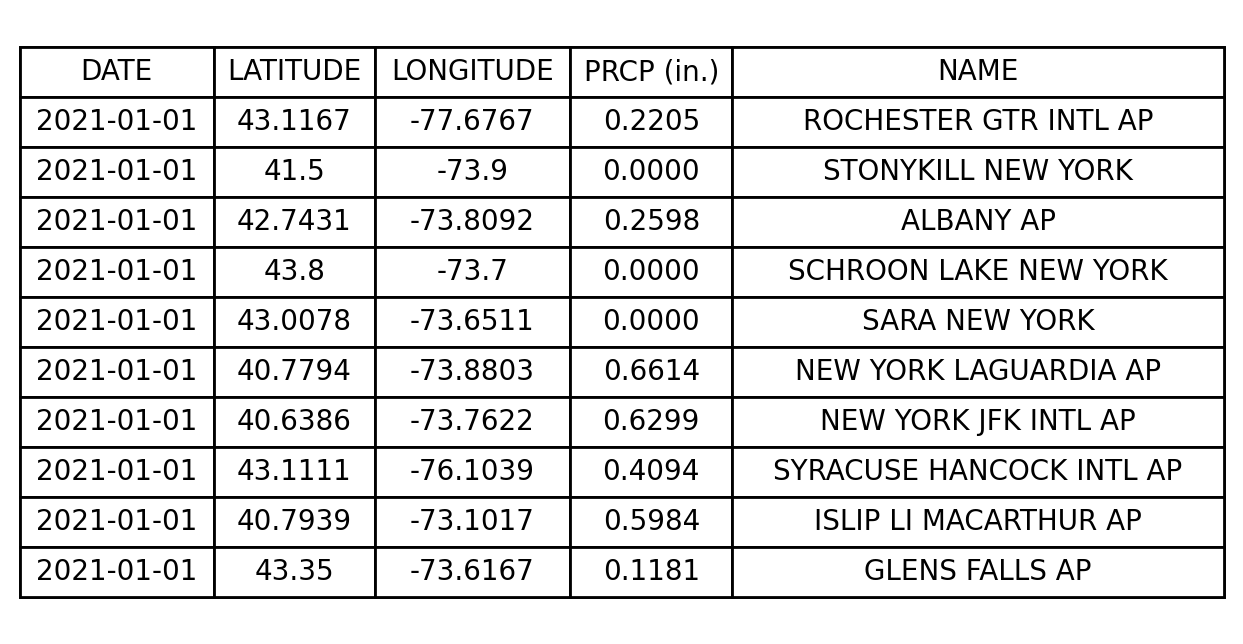
\includegraphics[width=.24\textwidth]{figures/intro/table.png} & 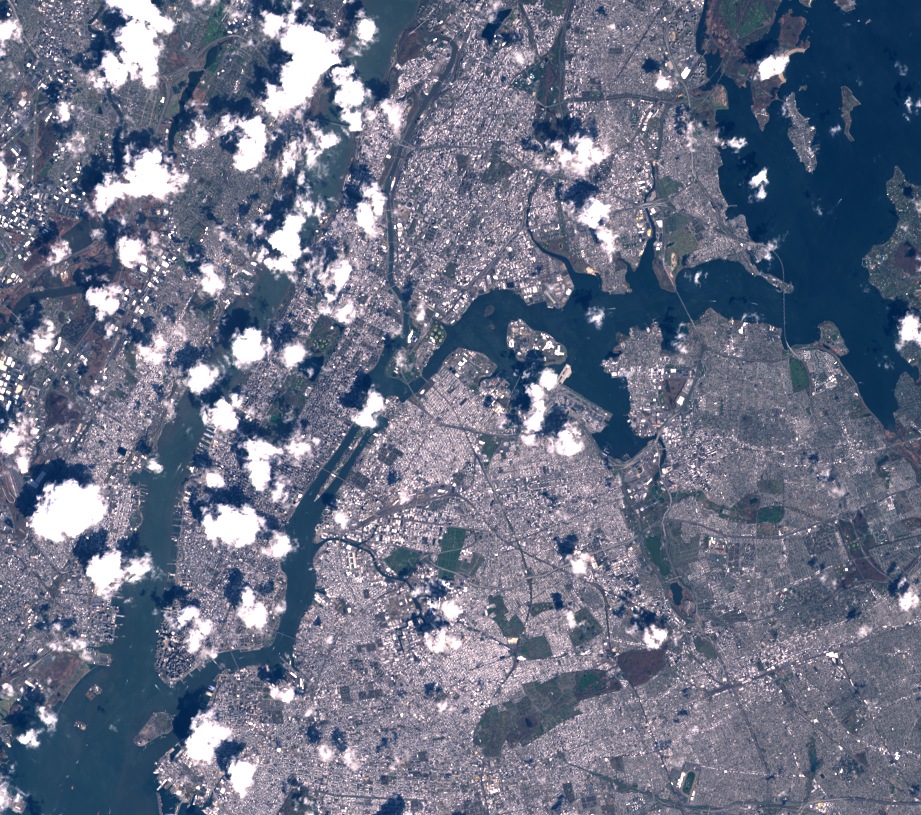
\includegraphics[width=.3\textwidth]{figures/intro/landsat.png} & 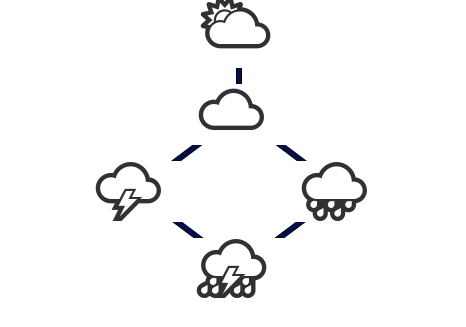
\includegraphics[width=.33\textwidth]{figures/math/graph.png} \\
            ggplot\cite{wickhamGgplot2ElegantGraphics2016a}  & ImageJ\cite{schneiderNIHImageImageJ2012}& Gephi\cite{bastianGephiOpenSource2009}\\
            Vega\cite{satyanarayanDeclarativeInteractionDesign2014} & ImagePlot\cite{studiesCulturevisImageplot2021} & Graphviz\cite{ellsonGraphvizOpenSource2002}\\
            Altair\cite{vanderplasAltairInteractiveStatistical2018}& Napari\cite{nicholas_sofroniew_2021_4533308} & Networkx\cite{HagbergExploringNetwork2008}\\
             Tableau \cite{StoltePolaris2002}& &\\
            \cite{hanrahanVizQL2006,MackinlayShowme2007}&&\\
           
        \end{tabular}
    \end{table}
\end{frame}

\begin{frame}{General purpose libraries generally can't\cite{toryRethinkingVisualizationHighlevel2004}}
    \begin{figure}
        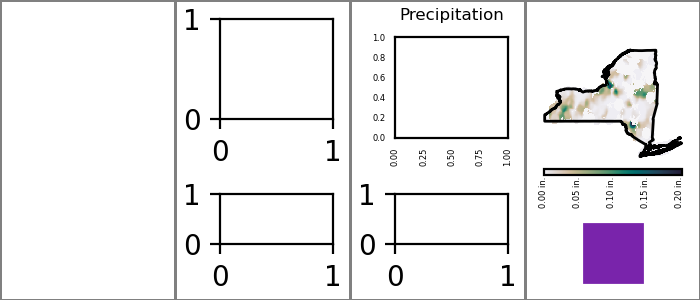
\includegraphics[height=.3\textheight]{../paper/figures/k_different_types.png}
    \end{figure}
    \begin{enumerate}
        \item Matplotlib\cite{hunterMatplotlib2DGraphics2007} $\rightarrow$Seaborn\cite{waskom2020seaborn}, xarray \cite{hoyer2017xarray} 
        \item D3 \cite{bostockDataDrivenDocuments2011}
        \item VTK \cite{hanwellVisualizationToolkitVTK2015,geveciVTK2012}(MayaVi\cite{RamachandranMayaVI2011})$\rightarrow$ Titan\cite{brianwylieUnifiedToolkitInformation2009}, ParaView\cite{ahrens2005paraview}
    \end{enumerate}
\end{frame}
\end{comment}
\subsection{Algebraic Topology & Category Theory}

\begin{frame}{Mathematical Data Abstraction}
    \begin{description}
        \item[Fiber Bundles] "unified, dimension-independent framework" that expresses data as the mapping between continuity and fields \cite{butlerVectorBundleClassesForm1992,butlerVisualizationModelBased1989}
        \item[Simplicial Databases] systemic way to apply a schema to a fiber, i.e. provides a way to name fields and bind them to types system (e.g. \texttt{int}, \texttt{float}) 
         \cite{spivakSIMPLICIALDATABASES, spivakDatabasesAreCategories2010} 
        \item[Sheaves on Bundles] "algebraic data structure" for representing data over topological spaces \cite{ghristElementaryAppliedTopology2014}
    \end{description}
\end{frame}

\begin{frame}{Fiber Bundles}
    \begin{columns}
        \column{0.39\textwidth}
            \begin{equation*}
                %\label{eq:related-work:continuity:fiber-bundle}
                \begin{tikzcd}[ampersand replacement=\&, row sep=huge]
                  \onslide*<2-|handout:2->{\dfiberc} \onslide*<4-|handout:4->{\arrow[r, hook]} \& \onslide*<3|handout:3->{\dtotalc} \onslide*<4-|handout:4->{\arrow[d, "\pi"']} \\
                   \& \onslide*<1-|handout:1->{\dbasec} \onslide*<5-|handout:5->{\arrow[u, "\dsectionc \in \cgamma{\dbasec}{\dtotalc}"', bend right, pos=.5]}
                \end{tikzcd}
            \end{equation*}
     \column{0.59\textwidth}
        \begin{description}
            \item<1-|handout:1->[\textcolor{base}{Base Space}] $( \dbasec, \mathcal{T})$, $\dbasepointc \in \opensetc \subset \dbasec$
            \item<2-|handout:2->[\textcolor{fiber}{Fiber Space}] $\dfiberc_{\dbasepointc} = \pi^{-1}(\dbasepointc)$
            \item<3-|handout:3->[\textcolor{total}{Total Space}]  $\dtotalc\restriction_{\opensetc} = \dbasec\restriction_{\opensetc} \times \dfiberc\restriction_{\opensetc}$ \\ for all $\opensetc \subset K$ 
        \end{description}
    \end{columns}
    \pause
    \begin{alertblock}<5-|handout:5->{Sections}
    $\cgamma{\opensetc}{\dtotalc\restriction_{\opensetc}} \coloneqq \big\{\dsectionc: \opensetc\rightarrow \dtotalc\restriction_{\openset} \; \bigm{\vert} \pi(\dsectionc(\dbasepointc)) = \dbasepointc\;for\, all\; \dbasepointc \in \opensetc \big\}$
    \end{alertblock}
\end{frame}

\subsection{Category Theory}
\begin{frame}{Category $\textcolor{source}{\mathcal{C}}$}
\begin{columns}
    \column{0.39\textwidth}
\begin{equation*}
    \begin{tikzcd}[ampersand replacement=\&]
        \textcolor{source}{C_1} \arrow[r, "f", color=source] \arrow[rd, "g\circ f"', color=source] \arrow["id_{C_1}"', loop, distance=2em, in=215, out=145, color=source] \& \textcolor{source}{C_2} \arrow[d, "g", color=source] \arrow["id_{C_2}"', loop, distance=2em, in=125, out=55, color=source] \\
    \& \textcolor{source}{C_3} \arrow["id_{C_3}"', loop, distance=2em, in=305, out=235, color=source]              
    \end{tikzcd}
    \end{equation*}
    \column{0.59\textwidth}
    \begin{alertblock}{associativity} 
        if $f: C_1 \rightarrow C_2$, $g: C_2 \rightarrow C_3$ and $h: C_3 \rightarrow C_4$ then $h\circ (g \circ f) = (h \circ g) \circ f$
    \end{alertblock}
    \begin{alertblock}{identity} 
        for every $f: C_1 \rightarrow C_2$ there exists identity morphisms $f \circ id_{C_1} = f = id_{C_2} \circ f$
    \end{alertblock}
    \end{columns}
\end{frame}
\begin{frame}{Category $\mathcal{\dbasec}$}
\begin{columns}
    \column{0.49\textwidth}
\begin{equation*}
    \begin{tikzcd}[ampersand replacement=\&]
        \textcolor{source}{C_1} \arrow[r, "f", color=source] \arrow[rd, "g\circ f"', color=source] \arrow["id_{C_1}"', loop, distance=2em, in=215, out=145, color=source] \& \textcolor{source}{C_2} \arrow[d, "g", color=source] \arrow["id_{C_2}"', loop, distance=2em, in=125, out=55, color=source] \\
    \& \textcolor{source}{C_3} \arrow["id_{C_3}"', loop, distance=2em, in=305, out=235, color=source]              
    \end{tikzcd}
    \end{equation*}
    \column{0.49\textwidth}
    \onslide<2-|handout:2->{
    \begin{tikzcd}[ampersand replacement=\&]
            \opensetc_1 \arrow[r, "\iota_{1,2}", color=base] \arrow[rd, "\iota_{1,2}\circ \iota_{2,3}"', color=base] \arrow["id_{\opensetc_1}"', loop, distance=2em, in=215, out=145, color=base] \& \opensetc_2 \arrow[d, "\iota_{2,3}", color=base] \arrow["id_{\opensetc_2}"', loop, distance=2em, in=125, out=55, color=base] \\
        \& \opensetc_3 \arrow["id_{\opensetc_3}"', loop, distance=2em, in=305, out=235, color=base]              
    \end{tikzcd}
    }
    \end{columns}
\end{frame}

\begin{frame}{Opposite Category $\textcolor{source}{\mathcal{C}^{op}}$}
    \begin{columns}
        \column{0.49\textwidth}
    \begin{equation*}
        \begin{tikzcd}[ampersand replacement=\&]
            \textcolor{fade}{C_1} \arrow[r, "f", color=fade] \arrow[rd, "g\circ f"', color=fade] \arrow["id_{C_1}"', loop, distance=2em, in=215, out=145, color=fade] \& \textcolor{fade}{C_2} \arrow[d, "g", color=fade] \arrow["id_{C_2}"', loop, distance=2em, in=125, out=55, color=fade] \\
        \& \textcolor{fade}{C_3} \arrow["id_{C_3}"', loop, distance=2em, in=305, out=235, color=fade]              
        \end{tikzcd}
        \end{equation*}
        \column{0.49\textwidth}
        \begin{equation*}
        \begin{tikzcd}[ampersand replacement = \&]
            \textcolor{source}{C_1} \arrow["id_{C_1}"', loop, distance=2em, in=215, out=145, color=source] \& \textcolor{source}{C_2} \arrow[l, "f"',color=source] \arrow["id_{C_2}"', loop, distance=2em, in=125, out=55, color=source]\\
            \& \textcolor{source}{C_3} \arrow[u, "g"', color=source] \arrow[lu, "f \circ g", color=source] \arrow["id_{C_3}"', loop, distance=2em, in=305, out=235, color=source]
            \end{tikzcd}
        \end{equation*}
        \end{columns}
\end{frame}

\begin{frame}{$\mathcal{C}^{op}$ with Objects of \setc}
    \begin{columns}
        \column{0.29\textwidth}
        \begin{tikzcd}[ampersand replacement=\&]
            \opensetc_1 \arrow[r, "\iota_{1,2}", color=base] \arrow[rd, "\iota_{1,2}\circ \iota_{2,3}"', color=base] \arrow["id_{\opensetc_1}"', loop, distance=2em, in=215, out=145, color=base] \& \opensetc_2 \arrow[d, "\iota_{2,3}", color=base] \arrow["id_{\opensetc_2}"', loop, distance=2em, in=125, out=55, color=base] \\
        \& \opensetc_3 \arrow["id_{\opensetc_3}"', loop, distance=2em, in=305, out=235, color=base]              
    \end{tikzcd}
        \column{0.69\textwidth}
        \onslide<2-|handout:2->{
            \begin{tikzcd}[ampersand replacement=\&]
            \cgamma{\opensetc_1}{\dtotalc\restriction_{\opensetc_1}} \&  \& \cgamma{\opensetc_2}{\dtotalc\restriction_{\opensetc_2}} \arrow[ll, "\iota^*\restriction_{\opensetc_1}"', color=set]\\
            \&\&\\\&  \& \cgamma{\opensetc_3}{\dtotalc\restriction_{\opensetc_3}} \arrow[uu, "\iota^*\restriction_{\opensetc_2}"', color=set] \arrow[lluu, "\iota^*\restriction_{\opensetc_2} \circ \iota^*\restriction_{\opensetc_1}", color=set]
            \end{tikzcd}


        }

        \end{columns}
\end{frame}

\begin{frame}{Functor $\textcolor{functor}{\bm{F}}: \textcolor{source}{\mathcal{C}} \rightarrow \textcolor{target}{\mathcal{D}}$}
\begin{columns}
    \column{.39\textwidth}
    \begin{equation*}
        \begin{tikzcd}[ampersand replacement = \&, ]
            \onslide*<1-|handout:1->{\textcolor{source}{c}} 
            \onslide*<1-|handout:1->{\arrow[d, "f"', shift right=0, color=source]} \onslide*<3-|handout:3->{\arrow[r, "F", color=functor]} \& 
            \onslide*<2|handout:2>{\textcolor{target}{d}}
            \onslide*<3-|handout:3->{\textcolor{target}{F(c)}} 
            \onslide*<2|handout:2>{\arrow[d, shift right=0, color=target]}
            \onslide*<3-|handout:3->{\arrow[d, "F(f)", shift right=0, color=target]} \\
            \onslide*<1-|handout:1->{\textcolor{source}{c^{\prime}}} 
            \onslide*<3-|handout:3->{\arrow[r, "F"', color=functor]}\& 
            \onslide*<2|handout:2>{\textcolor{target}{d^{\prime}}}
            \onslide*<3-|handout:3->{\textcolor{target}{F(c^{\prime})}}                      
        \end{tikzcd}
    \end{equation*}
    \column{.59\textwidth}
    \begin{alertblock}<4-|handout:4->{composition}
    $\textcolor{functor}{F}(\textcolor{source}{g}) \circ  \textcolor{functor}{F}(\textcolor{source}{f}) = \textcolor{functor}{F} (\textcolor{source}{g}\circ \textcolor{source}{f})$
    \end{alertblock}
    \begin{alertblock}<5-|handout:5->{identity}
    $\textcolor{functor}{F}(\textcolor{source}{id_c}) = \textcolor{target}{id}_{\textcolor{functor}{F}(\textcolor{source}{c})}$
    \end{alertblock}
\end{columns}
\end{frame}

\begin{frame}{Presheaf on Bundle: $\sheafc: \opensetc \textcolor{sheaf}{\rightarrow} \cgamma{\opensetc}{\dtotalc\restriction_{\opensetc}}$}
    \begin{columns}
    \column{0.29\textwidth}
    \begin{tikzcd}[ampersand replacement=\&, row sep=huge]
        \onslide*<8-|handout:8->{\dfiberc}
        \onslide*<8-|handout:8->{\arrow[r, hook]} \& 
        \onslide*<1-|handout:1->{\dtotalc}
        \onslide*<1-|handout:1->{\arrow[d, "\pi"']} \\
           \& 
        \onslide*<1-|handout:1->{\dbasec}
        \onslide*<3-|handout:3->{\arrow[u, "\dsectionc \in \cgamma{\dbasec}{\dtotalc}"', bend right, pos=.5]}
        \end{tikzcd}
    \column{0.69\textwidth}
        \begin{tikzcd}[ampersand replacement = \&, column sep=small]
            \onslide*<3-|handout:3->{{\cgamma{\opensetc_1}{\dtotalc\restriction_{{\opensetc_1}}}}} \& 
            {} \& 
            \onslide*<5-|handout:5->{{\cgamma{\opensetc_2}{\dtotalc\restriction_{\opensetc_2}}}} 
            \onslide*<6-|handout:6->{\arrow[ll, "\iota^*"', hook', color=set]} \\\& \&\\
            \onslide*<2|handout:2>{\opensetc_1 \subset \dbasec}
            \onslide*<3-|handout:3->{\opensetc_1} 
            \onslide*<4-|handout:4->{\arrow[uu, "\sheafc_{\dbasec}", color=sheaf]} 
            \onslide*<6-|handout:6->{\arrow[rr, "\iota"', hook, color=base]} \&   
            \onslide*<7-|handout:7->{\arrow[uu, "\sheafc_{\dbasec}" description, dotted, color=sheaf]} \& 
            \onslide*<5-|handout:5->{\opensetc_2} 
            \onslide*<5-|handout:5->{\arrow[uu, "\sheafc_{\dbasec}"', color=sheaf]}                   
            \end{tikzcd}
    \end{columns}
    \begin{description}
        \item<8-|handout:8->[stalk]$\sheafc(\dbasec)\restriction_{\dbasepointc}\coloneqq \lim\limits_{\opensetc\ni \dbasepointc} \Gamma(\opensetc, \dtotalc\restriction_{\opensetc}) \approx \dfiberc_{\dbasepointc}$
        \item<9-|handout:9>[germ]   $\dsectionc(\dbasepointc) \in \sheafc_{\dbasec}$
    \end{description}
\end{frame}

\begin{frame}{Sheaves}
    A sheaf is a presheaf that satisfies the following two axioms
    
    \onslide<2-|handout:2->{Given open cover $\mathcal{\opensetc} = \{\opensetc_i\}_{i\in I}$ of $\opensetc$:}
    \begin{block}<3-|handout:3->{locality}
    $\dsectionc^{1}, \dsectionc^{2} \in \sheafc(\opensetc_i)\\ \dsectionc^{1}\restriction_{\opensetc_i} = \dsectionc^{2}\restriction_{\opensetc_i} \implies \dsectionc^{1} = \dsectionc^{2}$
    \end{block} 
    \begin{block}<4-|handout:4>{gluing}
    $\dsectionc_{i} \in \sheafc(\opensetc_i), \dsectionc_{j} \in \sheafc(\opensetc_j), \opensetc_i, \opensetc_j \in \mathcal{U}\\ \dsectionc_{i}\restriction_{\opensetc_i\cap \opensetc_j} = \dsectionc_{j}\restriction_{\opensetc_i \cap \opensetc_j} \implies \dsectionc\restriction_{\opensetc_i} = \dsectionc_i$ 
    \end{block}      
\end{frame}

\begin{frame}{Morphism on Sheaves:\onslide<5-6,8-|handout:5-6,8->{ pullback}\onslide<8-|handout:8->{ and }\onslide<7-|handout:7->{pushforward}}
    \begin{equation*}
        \begin{tikzcd}[ampersand replacement=\&, row sep=huge]
            \onslide*<7-|handout:7->{\sheafc_{\gbasec}(\gbasec)} 
            \onslide*<7-|handout:7->{\arrow[rr, "\textcolor{functor}{\vindexpush}", color=functor]} \& \& 
            \onslide*<7-|handout:7->{(\textcolor{functor}{\vindexpush}\sheafc_{\gbasec})(\dbasec)}  \\
            \onslide*<2-|handout:2->{\gbasec}
            \onslide*<3-|handout:3->{\arrow[rr, "\vindex", color=functor]}
            \onslide*<7-|handout:7->{\arrow[u, "\sheaf_{\gbasec}", color=sheaf]}
            \onslide*<6,8-|handout:6,8->{\arrow[d, dashed, color=sheaf]} \&  \& 
            \onslide*<1-|handout:1->{\dbasec}
            \onslide*<4-6,8-|handout:4-6,8->{\arrow[d, "\sheaf_{\dbasec}", color=sheaf]}
            \onslide*<7-|handout:7->{\arrow[u, dashed, color=sheaf]} \\
            \onslide*<5-6,8-|handout:5-6,8->{(\textcolor{functor}{\vindexpull}\sheafc_{\dbasec})(\gbasec)} 
            \onslide*<5-6,8-|handout:5-6,8->{\arrow[rr, "\textcolor{functor}{\vindexpull}", color=functor]}  \& \& 
            \onslide*<4-6,8-|handout:4-6,8->{\sheafc_{\dbasec}(\dbasec)}                             
        \end{tikzcd}
    \end{equation*}
\end{frame}



\begin{frame}{Natural Transformation $\textcolor{nattran}{\alpha}: \textcolor{functor}{F} \textcolor{nattran}{\rightarrow} \textcolor{functor}{G}$}

    \adjustbox{scale=3, center}{
        \begin{tikzcd}[ampersand replacement=\&]
            \& {} \arrow[dd, "\alpha", Rightarrow, shorten=1.5em, color=nattran] \&             \\
          \textcolor{source}{\mathcal{C}} \arrow[rr, "F", bend left, color=functor] \arrow[rr, "G"', bend right, color=functor] \& \& \textcolor{target}{\mathcal{D}} \\
            \& {} \&            
          \end{tikzcd}}
    \end{frame}
    
    \begin{frame}{Natural Transformation $\textcolor{nattran}{\alpha}: \textcolor{functor}{F} \textcolor{nattran}{\rightarrow} \textcolor{functor}{G}$}
    \begin{equation*}
        \begin{tikzcd}[column sep=huge, ampersand replacement = \&]
            \textcolor{target}{F(c)} \arrow[dd, "F(f)"', color=target] \arrow[rr, "\alpha_{c}", bend left, color=nattran] \& \textcolor{source}{c} \arrow[dd, "f" description, color=source] \arrow[r, "G"', color=functor] \arrow[l, "F", color=functor] \& \textcolor{target}{G(c)} \arrow[dd, "G(f)", color=target] \\
            {} \arrow[rr, dotted, color=nattran] \& \& {}                      \\
            \textcolor{target}{F(c^{\prime})} \arrow[rr, "\alpha_{c^{\prime}}"', bend right, color=nattran] \& \textcolor{source}{c^{\prime}} \arrow[l, "F"', color=functor] \arrow[r, "G", color=functor] \& \textcolor{target}{G(c^{\prime})}          
        \end{tikzcd}
    \end{equation*}    
    \end{frame}

\begin{comment}

\subsection{Contributions}
\begin{frame}{Contributions}
    \begin{description}
        \item[Topological] continuity  
        \item[Equivariant] monoid action 
        \item[Artist] Matplotlib $\textit{artist}: \textit{data} \rightarrow \textit{graphic}$ 
        \item [Model] 
    \end{description}
\end{frame}

\section{Math}

\begin{frame}{Topological Equivariant Artist Model}
    \centering
    An artist $\mathscr{\vartist}$ is an equivariant map 
    \begingroup 
    \Huge
    \begin{equation*}
        \mathscr{\vartist}: \mathscr{\dtotal} \rightarrow \mathscr{\gtotal}
    \end{equation*}
    \endgroup
    from data $\mathscr{\dtotal}$ space to graphic $\mathscr{\gtotal}$ space. 
\end{frame}


\subsection{Data}
\begin{frame}{Model data as a fiber bundle \cite{butlerVectorBundleClassesForm1992,butlerVisualizationModelBased1989}}
    A fiber bundle is a tuple $(\dtotal,\,\dbase,\,\pi ,\,\dfiber)$ defined by the map $\pi$
    \begin{equation*}
        \label{eq:fiber_bundle}
        \begin{tikzcd}[ampersand replacement=\&]
            \dfiber \arrow[r, hook] \& \dtotal \arrow[r, "\pi"] \& \dbase
        \end{tikzcd}
    \end{equation*}
    \begin{description}
        \pause
        \item[total space \dtotal] topology
        \pause
        \item[fiber space \dfiber] schema
        \pause
        \item[base space \dbase] continuity
    \end{description}
\end{frame}

\begin{frame}{Encode variable types in a schema like fiber \cite{spivakDatabasesAreCategories2010,spivakSIMPLICIALDATABASES}}
    \begin{figure}[H]
        \centering
        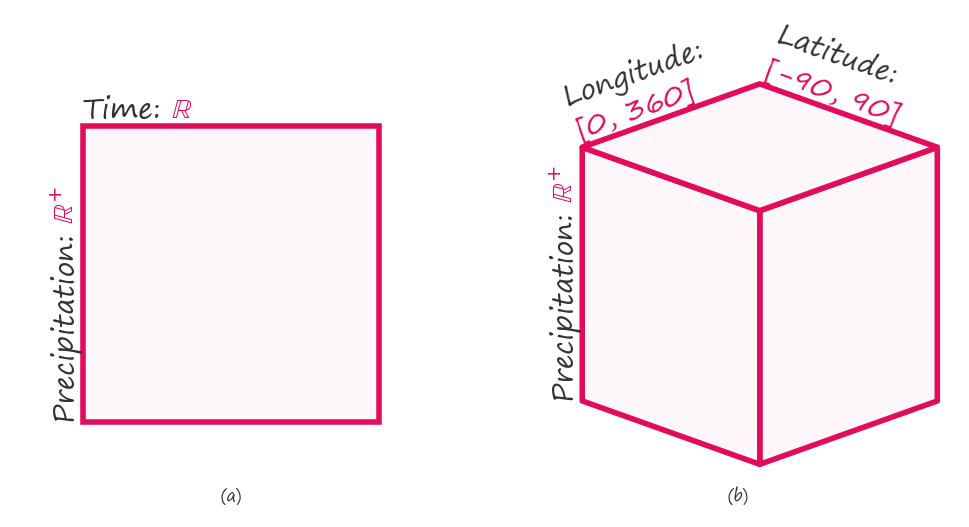
\includegraphics[width=\textwidth]{figures/math/fiber.png}
    \label{fig:data_fiber_example}
    \end{figure}
\end{frame}

\begin{frame}{Monoids are the structure of the components of \dfiber}
    \begin{figure}[H]
        \centering
        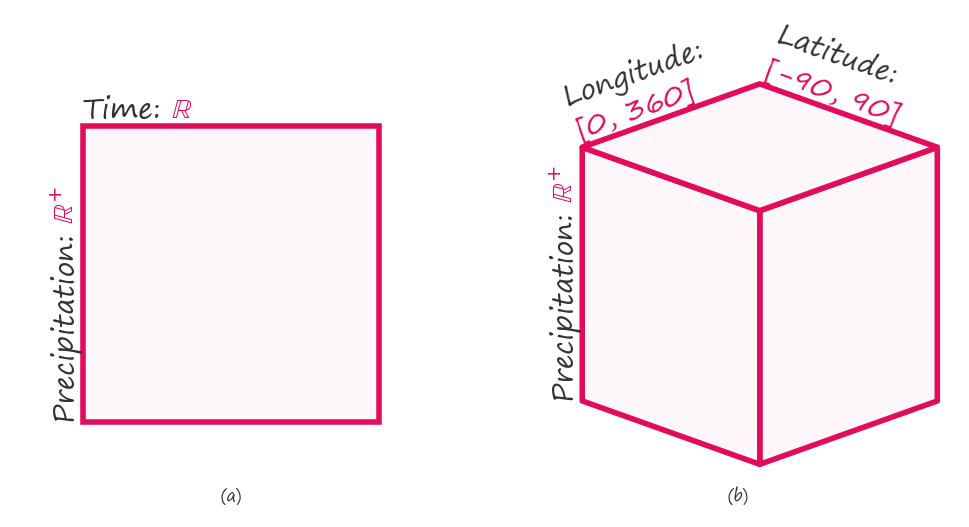
\includegraphics[height=.3\textheight]{figures/math/fiber.png}
    \label{fig:data_fiber_example}
    \end{figure}
        \begin{equation*}
            \dfiber = \dfiber_0 \times \ldots \times \dfiber_i \times \ldots \times \dfiber_n
        \end{equation*}
        \pause
        Monoid actions $\monoid_{i}$ (e.g. rotation, partial ordering) define the structure on $\dfiber_i$
        \begin{equation*}
            \bullet: \monoid_i\times \dfiber_i \rightarrow \dfiber_i
        \end{equation*}
        where $\bullet$ is associative and has an identity action. 
\end{frame}


\begin{frame}{\dbase\ is an indexing space}
    \begin{figure}[H]
        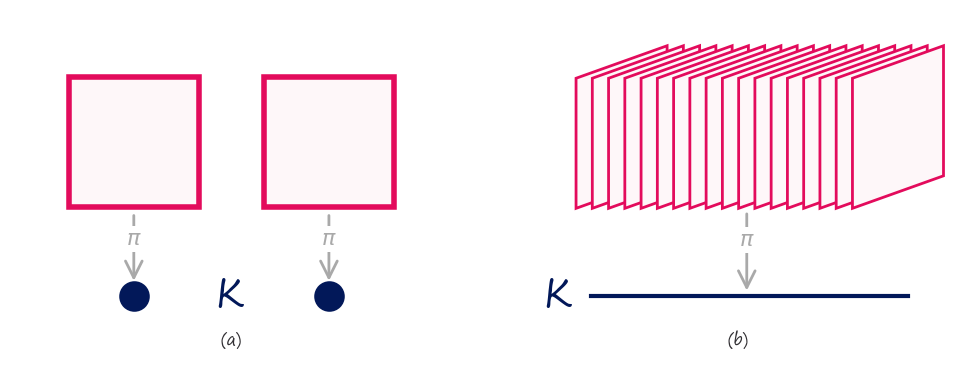
\includegraphics[width=1\textwidth]{figures/math/base.png}
    \label{fig:base_example}
    \end{figure}
\end{frame}



\begin{frame}{Data are sections \dsection\ on \dtotal}
    For any fiber bundle, there exists a map
    \begin{equation*}
        \begin{tikzcd}[ampersand replacement=\&]
            \dfiber \arrow[r, hook] \& \dtotal \arrow[d, "\pi"'] \\
                              \& \dbase \arrow[u, "\dsection"', bend right]
        \end{tikzcd}
    \end{equation*}
     s.t. $\pi(\dsection(\dbasepoint)) = \dbasepoint$. $\Gamma(\dtotal)$ is the set of all global sections.
     \begin{figure}[H]
        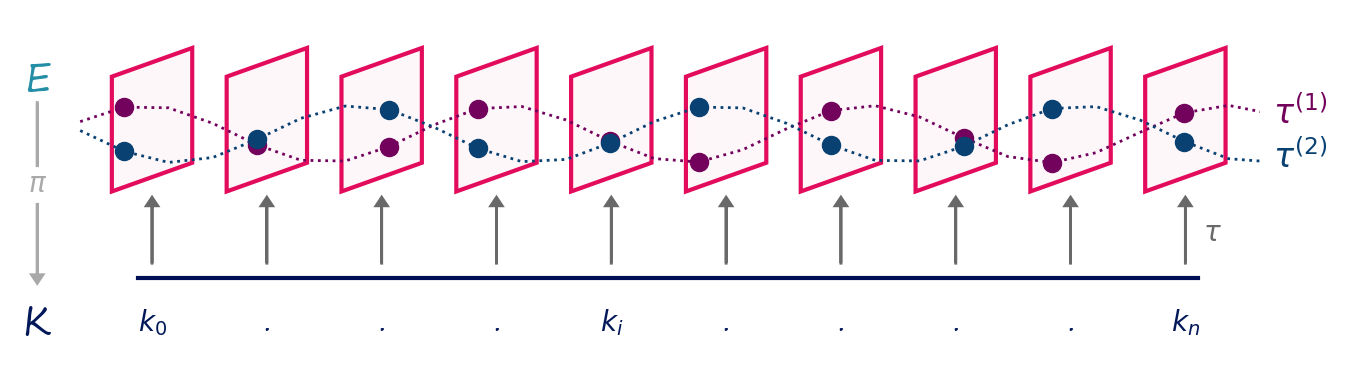
\includegraphics[width=1\linewidth]{figures/math/fiberbundle.png}
        \label{fig:data_sections}
    \end{figure}
\end{frame}


\subsection{Graphic}
\begin{frame}{Graphic Bundle $(\gtotal,\,\gbase,\,\pi ,\,\gfiber)$} % watch dr explaination
    \only<2->{Continuity is preserved via the many \gbasepoint\ to one \dbasepoint\ map $\vindex: \gbase\rightarrow\dbase$}

    \only<1>{
        \begin{equation*} 
            \begin{tikzcd}[ampersand replacement=\&]
                F \arrow[r, hook] \& E \arrow[d, "\pi"']              \& D \arrow[r, hook] \& H \arrow[d, "\pi"']              \\
                                  \& K \arrow[u, "\tau"', bend right] \&                   \& S \arrow[u, "\rho"', bend right]
                \end{tikzcd}
            \end{equation*}}
    \only<2->{
    \begin{equation*} 
        \begin{tikzcd}[ampersand replacement=\&]
            F \arrow[r, hook] \& E \arrow[d, "\pi"']              \& D \arrow[r, hook] \& H \arrow[d, "\pi"']                                 \\
                              \& K \arrow[u, "\tau"', bend right] \&                   \& S \arrow[ll, "\xi"'] \arrow[u, "\rho"', bend right]
            \end{tikzcd}
        \end{equation*}}
    \only<3->{   
    \gfiber\ is a proxy for the target display, for example $(x,\, y,\, r,\, g,\, b) \in \gfiber$}
    \pause
    \begin{figure}[H] %%%bring up one at a time
        \begin{overprint}
            \onslide<4|handout:0>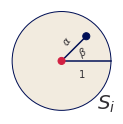
\includegraphics[width=1\linewidth]{figures/math/scatter_s.png}
            \onslide<5|handout:0>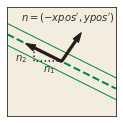
\includegraphics[width=1\linewidth]{figures/math/line_s.png}
            \onslide<6>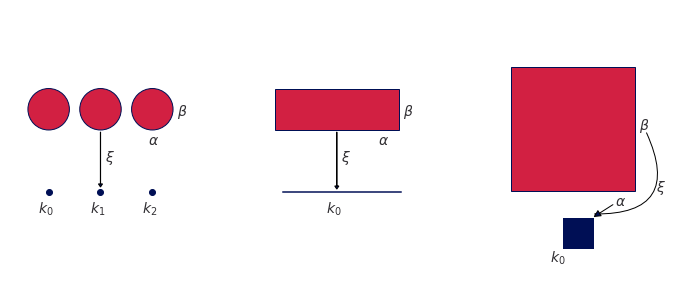
\includegraphics[width=1\linewidth]{figures/math/image_s.png}
        \end{overprint}
    \end{figure}
\end{frame}

\subsection{Artist}
\begin{frame}{Visual bundle $(\vtotal,\,\dbase,\,\pi ,\,\vfiber)$}
    \begin{equation*}
        \mathcal{A}:\mathcal{E}\rightarrow\mathcal{H}
    \end{equation*}
\pause
\begin{equation*}
    \label{eq:artist_diagram}
    \begin{tikzcd}[ampersand replacement=\&]
        \dtotal^{\prime} \arrow[r, "\vchannel"] \arrow[rd, "\pi"'] \& \vtotal \arrow[d, "\pi"] \& \vindex^*\vtotal \arrow[r, "\vmark"] \arrow[d, "\vindex^*\pi"'] \arrow[l, "\vindex^*"'] \& \gtotal \arrow[ld, "\pi"] \\
                                              \& \dbase                  \& \gbase \arrow[l, "\vindex"']                                              \&                    
        \end{tikzcd}
\end{equation*}
\pause
\begin{equation*}
    \vartist: \mathcal{O}(\dtotal) \rightarrow \mathcal{O}(\gtotal)
\end{equation*}
\end{frame}

\begin{frame}{Visualization Assembly Function}
    \begin{figure}
        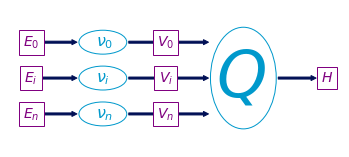
\includegraphics[width=\textwidth]{figures/math/path_of_q.png}
    \end{figure}
    \pause
    \begin{equation*}
        \label{eq:nu_expanded}
        \{\vchannel_{0}, \ldots, \vchannel_{n}\}: \{\dsection_{0}, \ldots, \dsection_{n}\} \mapsto \{\vsection_{0}, \ldots, \vsection_{n}\}
    \end{equation*}
    \pause
    \begin{equation*}
        Q = \nu \circ \tau
    \end{equation*}
\end{frame}


\begin{frame}{Group Equivariance: Stevens' Scales \cite{stevensTheoryScalesMeasurement1946}}
\begin{table}[H]
    \begin{tabularx}{\textwidth}{|l|l|X|}\toprule
        \textbf{scale} & \textbf{group} & \textbf{constraint} \\\midrule
        nominal & permutation &  $\text{if } \delement_1 \neq \delement_2 \text{ then } \vchannel (\delement_1) \neq\vchannel(\delement_2)$\\
        ordinal &  monotonic & $\text{if } \delement_1 \leq \delement_2 \text{ then } \vchannel (\delement_1) \leq \vchannel(\delement_2)$\\
        interval &  translation &  $\vchannel (x + c) = \vchannel(x) + c$ \\
        ratio &  scaling &  $\vchannel(xc) = \vchannel(x)*c $\\ \bottomrule
    \end{tabularx}
\end{table}
\end{frame}

\begin{frame}{Monoid Equivariance: Partial Orders}
    \begin{figure} 
        \begin{overprint}
            \onslide<1|handout:0>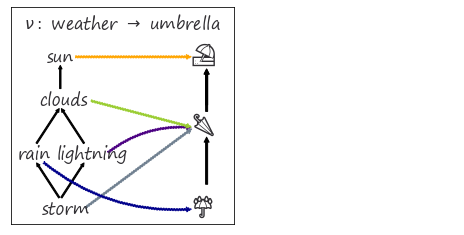
\includegraphics[width=1\linewidth]{figures/math/partial.png}
            \onslide<2|handout:0>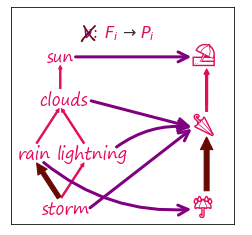
\includegraphics[width=1\linewidth]{figures/math/partial_invalid.png}
            \onslide<3>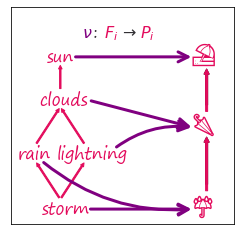
\includegraphics[width=1\linewidth]{figures/math/partial_fixed.png}
        \end{overprint}
    \end{figure}
\end{frame}


\begin{frame}{Visualization Equivariance}
    \begin{figure}[H]
        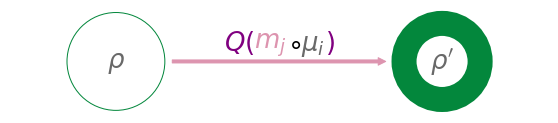
\includegraphics[width=\textwidth]{figures/math/diff_type_q.png}
    \end{figure}
    \begin{equation*}
        \vmark(\vsection) = \vmark(\vsection^{\prime})\implies \vmark(m\circ\vsection) = \vmark(m\circ\vsection^{\prime})
    \end{equation*}
  
\end{frame}

\begin{frame}{Scatter: $\vmark(xpos, ypos)(\alpha, \beta)$}
    \begin{figure}[H]
        \begin{overprint}
            \onslide<1|handout:0>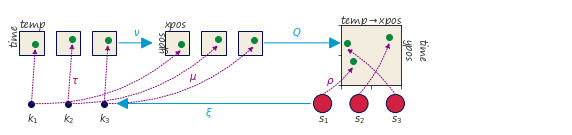
\includegraphics[width=1\linewidth]{figures/math/scatter_q.png}
            \onslide<2|handout:0>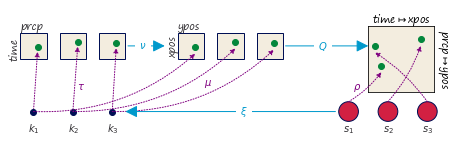
\includegraphics[width=1\linewidth]{figures/math/scatter_with_s.png}
        \end{overprint}
    \end{figure}   
\end{frame}

\begin{frame}{Line: $\vmark(xpos, \hat{n_{1}}, ypos, \hat{n_{2}})(\alpha, \beta)$ }
    \begin{figure}[H]
        \begin{overprint}
            \onslide<1|handout:0>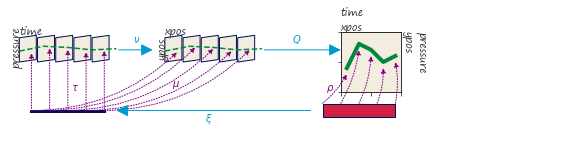
\includegraphics[width=1\linewidth]{figures/math/line_q.png}
            \onslide<2|handout:0>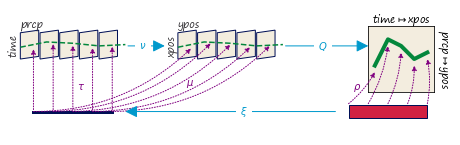
\includegraphics[width=1\linewidth]{figures/math/line_with_s.png}
        \end{overprint}
    \end{figure}   
\end{frame}

\begin{frame}{Image $\vmark(xpos, ypos, color)$}
    \begin{figure}[H]
        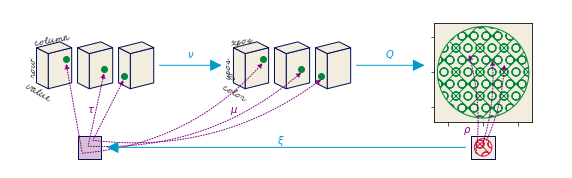
\includegraphics[width=1\textwidth]{figures/math/image.png}
    \end{figure}
\end{frame}

\begin{frame}{Build \vmark\ over \dbase: \vmarkd}
\begin{figure}[H]
    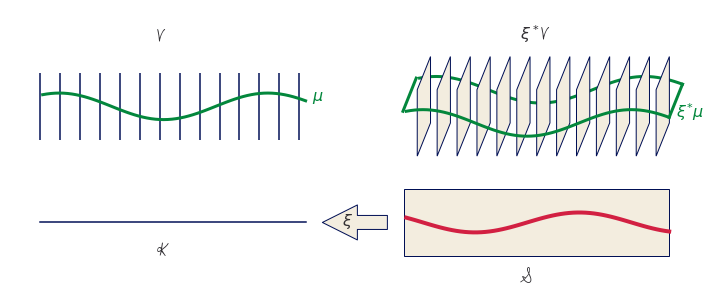
\includegraphics[width=1\textwidth]{figures/math/q_hat.png}
\end{figure}
\begin{equation*}\label{eq:qhat_q_s}
    \vmarkd(\vsection(\dbasepoint))(\gbasepoint) \coloneqq \vmark((\vsectionpull)(\gbasepoint))
\end{equation*} 
\end{frame}

\begin{frame}{Composition of artists $+ \coloneqq \sqcup \dtotal_{i}$} 
    \begin{figure}
        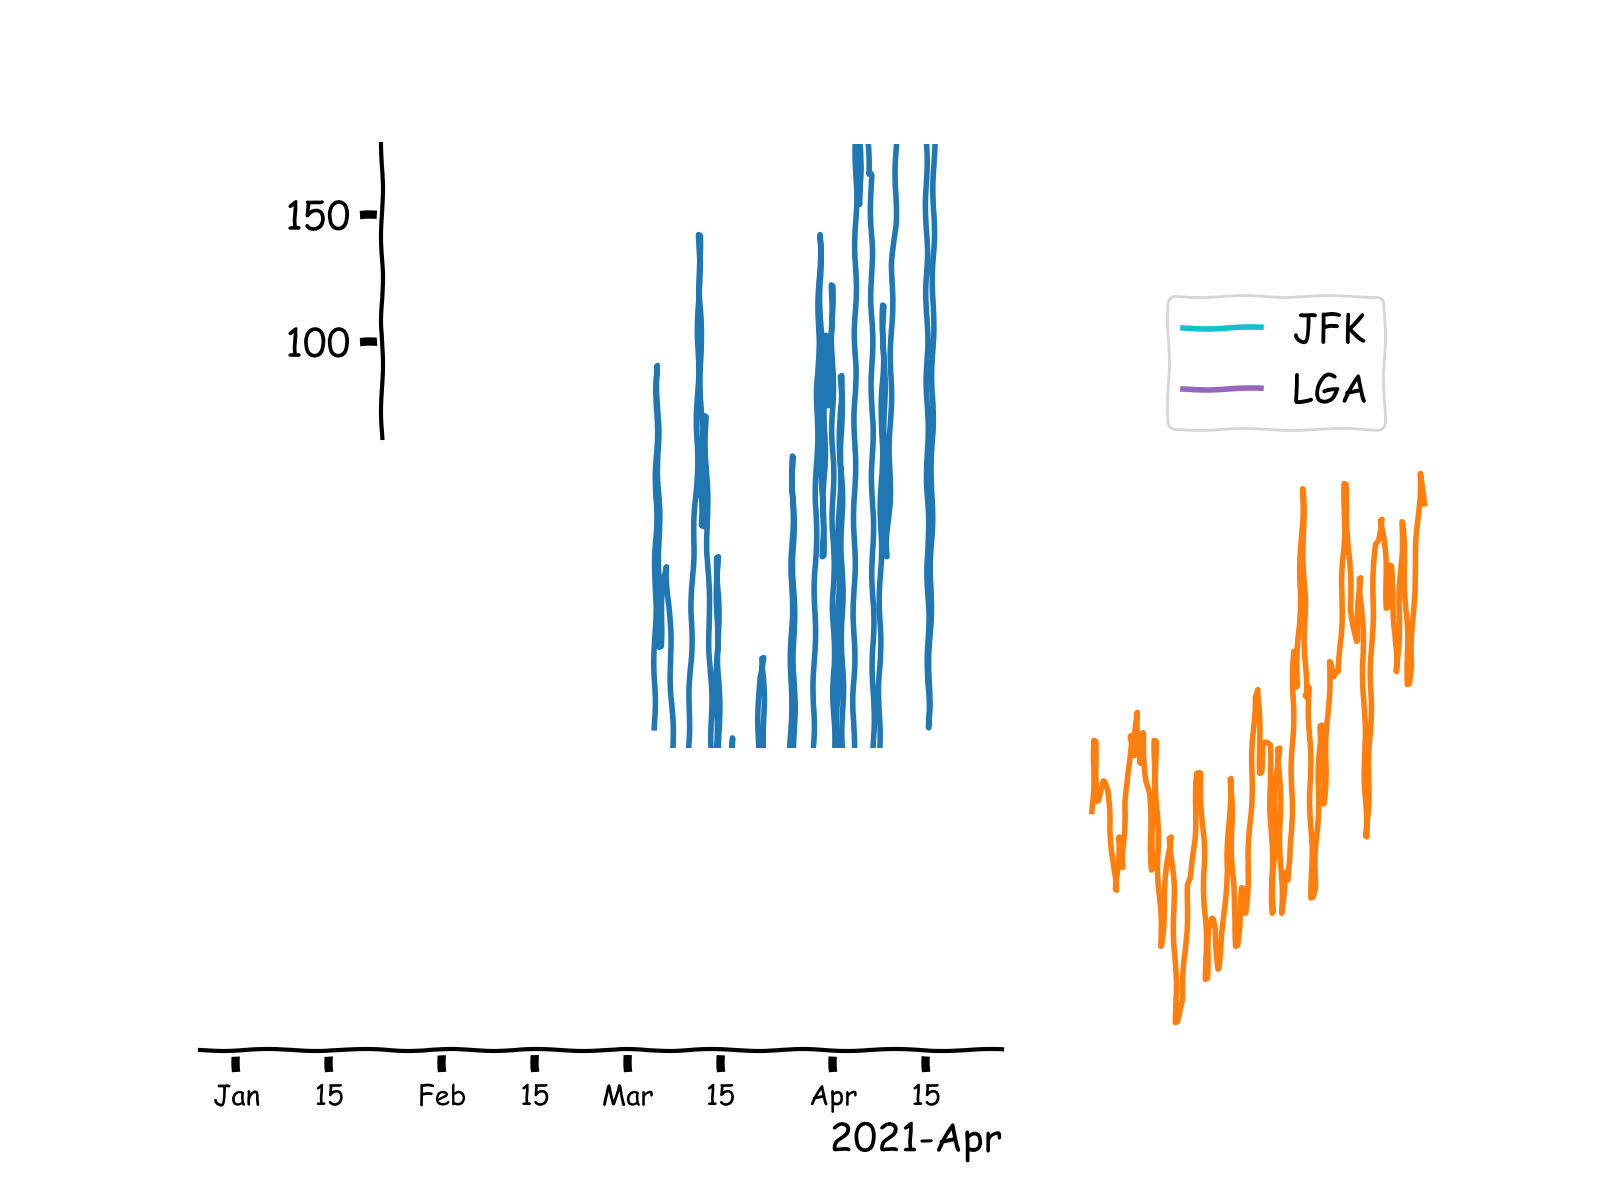
\includegraphics[width=1\textwidth]{figures/math/exploding_artist.png}
    \end{figure}
\end{frame}


\section{Code}
\begin{frame}{TEAM driven rearchitecture of Matplotlib}
    \begin{itemize}
        \item complex visualizations
        \pause 
        \item structure preserving maps from data to visual
        \begin{itemize}
            \item data and graphics have equivalent continuity
            \item properties are equivariant under monoid actions
        \end{itemize}  
        \pause
        \item fiber bundles are an abstraction
        \begin{itemize}
            \item topologically complex heterogenous data 
            \item target display spaces
        \end{itemize}
    \end{itemize}
\end{frame}

\begin{frame}[fragile]{How do we make things?}
    \begin{figure}[H]
        \begin{subfigure}{0.49\textwidth}
            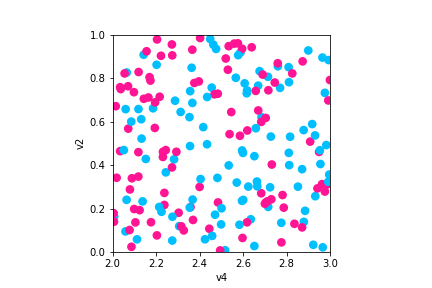
\includegraphics[width=\textwidth]{figures/code/scatter_0.png}
        \end{subfigure}
        \begin{subfigure}{0.49\textwidth}
            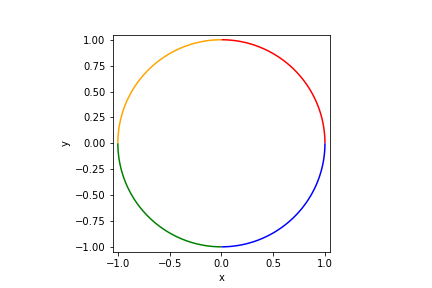
\includegraphics[width=\textwidth]{figures/code/line_1.png}
        \end{subfigure}
    \end{figure}
    \begin{columns}
    \column{0.49\textwidth}
    \begin{minted}{python}
    fig, ax = plt.subplots()
    artist = Point(data, transforms)
    ax.add_artist(artist)
    \end{minted}
    \column{.49\textwidth}
    \begin{minted}{python}
    fig, ax = plt.subplots()
    artist = Line(data, transforms)
    ax.add_artist(artist)
    \end{minted}
    \end{columns}
\end{frame}

\subsection{Artist}
\begin{frame}[fragile]{ \vchannel}
    \begin{minted}{python}
    cmap =  color.Categorical({'true':'deeppink', 'false':'deepskyblue'})
    transforms = {'x': {'name': 'v4', 'encoder': lambda x: x},
                    'y': {'name': 'v2', 'encoder': lambda x: x},
                    'facecolors': {'name':'v3', 'encoder': cmap}, 
                    's':{'name': None , 
                        'encoder': lambda _: itertools.repeat(.02)}}
    \end{minted}
    \begin{itemize}
        \item \mintinline{python}{lambda x: x} is identity \vchannel\
        \item \mintinline{python}|{'name':None}| map into \vfiber\ without corresponding \dsection\
        \item \mintinline{python}{color.Categorical} is custom \vchannel
    \end{itemize}
\end{frame}
    
\begin{frame}[fragile]{\vartist} %% rewrite w/ letters in talk
    \begin{minted}{python}
        class ArtistClass(matplotlib.artist.Artist):
            def __init__(self, E, V, *args, **kwargs):
                # set properties that are specific to the artist
                # stash the input E and V
                super().__init__(*args, **kwargs)
        
            def qhat(self, **args):
                # set the properties of the graphic
        
            def draw(self, renderer):
                # returns tau, indexed on fiber then key 
                tau = self.E.view(self.axes) 
                # visual channel encoding applied fiberwise 
                visual = {p_i: nu_i(tau_i)
                          for p_i, nu_i, tau)i 
                          in zip(self.V, tau)}
                self.qhat(**visual)
                # pass configurations off to the renderer
                super().draw(renderer)
        \end{minted}
\end{frame}

\begin{frame}[fragile]{\vmarkd}
\begin{minted}{python}
    class Point(mcollections.Collection):
        def assemble(self, x, y, s, facecolors='C0' ):
            # construct geometries of the circle glyphs in visual coordinates
            # set attributes of glyphs

    class Line(mcollections.LineCollection):
        def assemble(self, x, y, color='C0'):
            # assemble line marks as set of segments 
    \end{minted}
\end{frame}

\subsection{Data}
\begin{frame}[fragile]{Continuity}
    \begin{minted}{python}
class PointData: 
    # Fiberbundle is consistent across all sections
    FB = FiberBundle({'tables': ['vertex']},  
        {'v1': float, 'v2': str, 'v3': float})
    def tau(self, k):
        return # tau evaluated at one point k

class LineData: 
    FB = FiberBundle({'tables': ['edge']},
                {'x' : float, 'y':  float, 'color':mtypes.Color()})
    def tau(self, k): 
        return # tau evaluated on interval k
    \end{minted}
\end{frame}

\begin{frame}[fragile]{Same Artist, Different \dtotal}
    \begin{figure}[H]
        \begin{subfigure}{0.49\textwidth}
            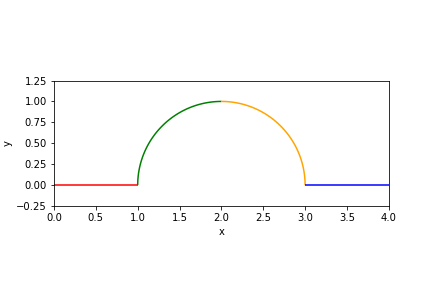
\includegraphics[width=\textwidth]{figures/code/linec_1.png}
        \end{subfigure}
        \begin{subfigure}{0.49\textwidth}
            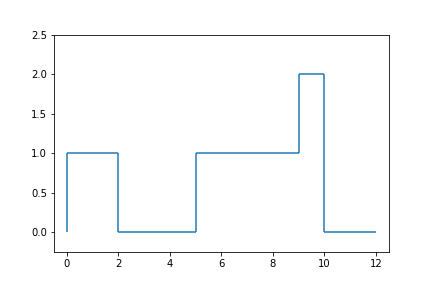
\includegraphics[width=\textwidth]{figures/code/lined_1.png}
        \end{subfigure}
    \end{figure}
\begin{minted}{python}
LineData(FB, edge_table, vertex_table, connect=True)
LineData(FB, edge_table, vertex_table, num_samples=2, connect=False)
\end{minted}
\end{frame}

\begin{frame}{Proposed Work}
\begin{figure}
    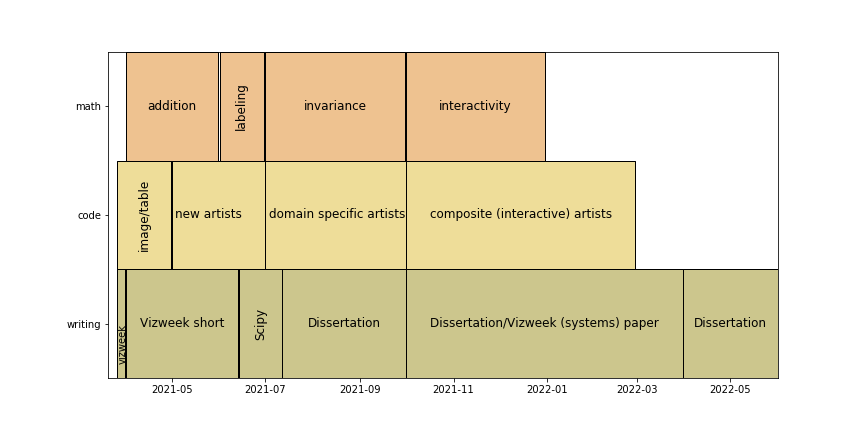
\includegraphics[width=1\textwidth]{figures/intro/gantt.png}
\end{figure}
\end{frame}

\begin{frame}{Acknowledgments}
    \begin{itemize}
        \item Professor Michael Grossberg and Dr. Thomas Caswell
        \item Professor Haralick, Professor Vo, Professor Manovich, Dr. Hanwell
        \item Matplotlib development team 
        \item CZI EOSS (grant number 2019-207333) from the Chan Zuckerberg Initiative DAF, an advised fund of Silicon Valley Community Foundation
    \end{itemize}
    
\end{frame}

\begin{frame}[allowframebreaks]{References}
\printbibliography
\end{frame}
\appendix 

\begin{frame}{Bertin Retinal Variables}
    \begin{figure}
        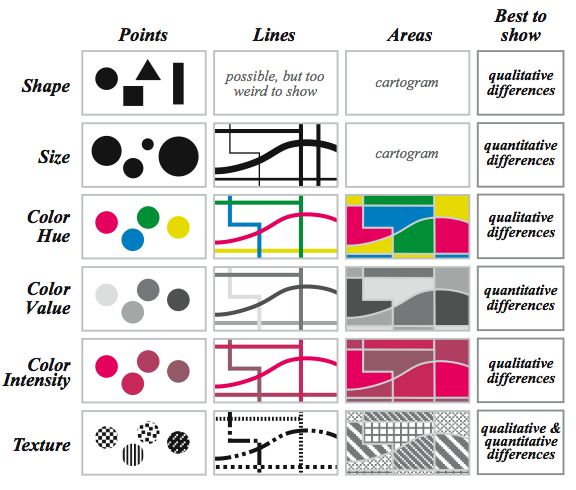
\includegraphics[width=.7\textwidth]{figures/intro/retinal_variables.png}
        \caption{This tabular form of Bertin's retinal variables is from Understanding Graphics \cite{malamedInformationDisplayTips2010} who reproduced it from Krygier and Wood's \textit{Making Maps: A Visual Guide to Map Design for GIS}\cite{krygierMakingMapsVisual2005}}
    \end{figure}
\end{frame}


\begin{frame}{Fiber is all possible values a variable can be \cite{spivakDatabasesAreCategories2010,spivakSIMPLICIALDATABASES}}
    Given a space of all possible values \ftotal\
    \begin{equation*}
        \label{eq:data_types}
        \begin{tikzcd}[ampersand replacement=\&]
            \fttype \arrow[r] \arrow[d, "\pi_{\fsection}"'] \& \ftotal \arrow[d, "\pi"] \\
            \fnames \arrow[r, "\fsection"']                  \& \ftypes       
        \end{tikzcd}
    \end{equation*}
    a fiber component is the restricted space $\ftotal_{\fsection(\fname)}$. 
    \begin{equation*}
        \dfiber = \ftotal_{\fsection(\fname)} = \ftotal_{\ftype} 
    \end{equation*}
    \begin{description}
        \item[\ftypes] data types of the variables in the dataset 
        \item[\ftotal] disjoint union of all values of type $\ftype \in \ftypes$ 
        \item[\fnames] variable names, $\fname \in \fnames$
        \item[\fttype] \ftotal\ restricted to the data type of a named variable   
    \end{description}
\end{frame}

\begin{frame}{Monoid actions}
    A monoid \monoid\ is a set with
    \begin{description}
        \item[associative binary operator] $\ast:\monoid \times \monoid\rightarrow \monoid$
        \item[identity element] $e\in \monoid$ such that $e\ast a= a \ast e = a$ for all $a \in \monoid$. 
    \end{description}
    \begin{block}{left monoid action}
    A set \dfiber\ with an action\cite{nlab:action} $\bullet: \monoid\times \dfiber \rightarrow \dfiber$ with the properties:
        \begin{align*}
            \textbf{associativity}\;& \text{for all } f,g \in \monoid \text{ and } x\in \dfiber,\, f\bullet(g\bullet x) = (f\ast g) \bullet x\\
            \textbf{identity}\;& \text{for all } x\in \dfiber, e\in \monoid,\,  e\bullet x = x 
        \end{align*}
    \end{block}
\end{frame}

\begin{frame}{Keeping track of sections with sheafs}
    Restriction maps of a sheaf describe how local $\iota^*\dsection$ can be glued into larger sections \cite{ghristElementaryAppliedTopology2014,ghristHomologicalAlgebraData2018}
    \begin{equation*}
        \label{eq:sheaf}
        \begin{tikzcd}[ampersand replacement=\&]
            \iota^*\dtotal \arrow[d, "\pi"'] \arrow[r, "\iota^*", hook]             \& \dtotal \arrow[d, "\pi"']                  \\
            U \arrow[r, "\iota", hook] \arrow[u, "\iota^{*}\dsection"', bend right] \& \dbase \arrow[u, "\dsection"', bend right]
        \end{tikzcd}
    \end{equation*}
    The inclusion map $\iota: U \rightarrow \dbase$ pulls \dtotal\ over $U$ such that the pulled back $\iota^*\dsection$ only contains records over $U \subset \dbase$.
\end{frame}

\begin{frame}{Rendering: Define a Pixel}
    \begin{columns}
        \column{0.5\textwidth}
        Given a pixel
        \begin{equation*}
        p=\left[y_{top}, y_{bottom}, x_{right}, x_{left}\right]
        \end{equation*}
        the inverse map of the bounding box 
        \begin{equation*}
        \gbase_{p} ={\gsection_{xy}}^{-1}(p)
        \end{equation*}
        is a region $\gbase_p \subset \gbase$ such that 
        \begin{align}
            \scriptstyle r_p &= \scriptstyle \iint\limits_{S_p} \rho_r(s)ds^{2}\\
            \scriptstyle g_p &= \scriptstyle \iint\limits_{S_p} \rho_g(s)ds^{2}\\
            \scriptstyle  b_p &= \scriptstyle \iint\limits_{S_p} \rho_b(s)ds^{2}
        \end{align}
        yields the color of the pixel. 
        \column{0.5\textwidth}
        \begin{figure}[H]
            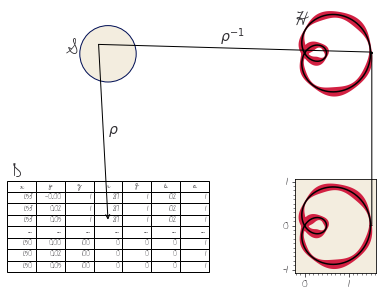
\includegraphics[width=\textwidth]{figures/math/render.png}
        \end{figure}
    \end{columns}
\end{frame}

\begin{frame}{$\mathcal{A}:\mathcal{E}\rightarrow\mathcal{E}$}
    The topological artist is a sheaf map
    \begin{equation*}
    \vartist: \mathcal{O}(\dtotal) \rightarrow \mathcal{O}(\gtotal)
    \end{equation*}
    that carries homomorphism of monoid actions $\varphi: \monoid \rightarrow \monoid^{\prime}$ 
    \cite{cegarraCohomologyMonoidsOperators2019} 
    \begin{equation*}
    \vartist(m\cdot \delement) = \varphi(m)\cdot \vartist(\delement) 
    \end{equation*}
\end{frame}

\begin{frame}{Visual Channel Encoders}
    We define the visual transformers \vchannel\ on components of the data bundle $\dsection_{i}$
    \begin{equation*}
        \label{eq:nu_expanded}
        \{\vchannel_{0}, \ldots, \vchannel_{n}\}: \{\dsection_{0}, \ldots, \dsection_{n}\} \mapsto \{\vsection_{0}, \ldots, \vsection_{n}\}
    \end{equation*}
    as the set of equivariant maps with the constraint 
    \begin{equation*}
        \vchannel_i(m_{\delement}(\dtotal_i)) = \varphi(m_{\delement})(\vchannel_i(\dtotal_i))
    \end{equation*} 
    where $\varphi:\monoid\rightarrow \monoid^{\prime}$ carries a homomorphism of monoid actions. 
\end{frame}

\begin{frame}{\vfiber\ Components}    
\begin{table}[H]
    \renewcommand{\arraystretch}{2}
    \begin{tabulary}{\textwidth}{|l|L|l|}\hline
     $\bm{\vchannel_{i}}$                      & $\bm{\vsection_{i}}$                                                            & $\bm{codomain(\vchannel_{i}) \subset \vfiber_{i}}$  \\ \hline                                              
    position                    & x, y, z, theta, r                                                          & $\mathbb{R}$   \\ \hline
    size                        & linewidth, markersize                                            & $\mathbb{R}^{+}$   \\ \hline
    shape                       & markerstyle                                                      & $\{f_{0}, \ldots, f_{n}\}$ \\ \hline
    color                       & color, facecolor, markerfacecolor, edgecolor  & $\mathbb{R}^{4}$ \\ \hline
    \multirow{2}{*}{texture}    & hatch                                                            & $\mathbb{N}^{10}$\\\cline{2-3}
                                & linestyle                                                        & $(\mathbb{R}, \mathbb{R^+}^{n, n\%2=0})$ \\ \hline              
    \end{tabulary}
    \label{tab:mpl_visual_variable_fiber}
\end{table}
\end{frame}
\begin{frame}{Monoid Equivariance: Partial Orders}
    \begin{figure} %break out steps/reveal
        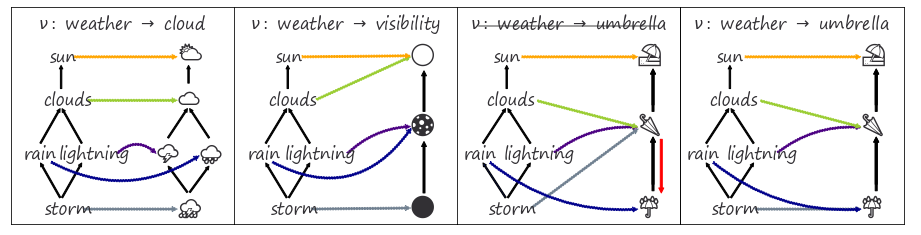
\includegraphics[width=1\textwidth]{figures/math/monoid_equivariant.png}
    \end{figure}
\end{frame}

\begin{frame}{Glyph}
    The glyph is the graphic generated by $\vmark(\gbase_{\dbasepathpoint})$ where the path connected components $\dbasepath \subset \dbase$ are defined 
    \begin{equation*}
    \dbasepath = \{\dbasepathpoint \in \dbase \text{ s. t. } \exists \gamma \text{ s.t. } \gamma(0)=\dbasepoint \text{ and }\gamma(1)=\dbasepathpoint\}
    \end{equation*}
    such that the  path $\gamma$ from \dbasepoint\ to \dbasepathpoint\ is a continuous function from the interval [0,1] and $\gbase_{\dbasepathpoint}$ is the region
    \begin{equation*}
        \begin{tikzcd}[ampersand replacement=\&]
            \gtotal \arrow[r, shift left] \& \gbase_\dbasepathpoint \arrow[rr, "\vindex(\gbasepoint)", shift left] \arrow[l, "\gsection(\gbase_\dbasepathpoint)"] \& \& \dbasepath_{\dbasepoint} \arrow[ll, "\vindex^{-1}(\dbasepath)"]
            \end{tikzcd}
        \label{eq:mark}
    \end{equation*}
    such that the glyph is differentiable, in keeping with Ziemkiewicz and Kosara's description of a glyph\cite{ziemkiewiczEmbeddingInformationVisualization2009}.
\end{frame}

\begin{frame}{Artist Equivalance class}
    When artists share a base space 
    \begin{equation*}
        \dbase_2 \hookrightarrow \dbase_1
    \end{equation*}
    a composition operator can be defined such that the the artists can be considered to be acting on different components of the same section. 
\end{frame}

\begin{frame}[fragile]{Complex \vchannel}
    \begin{minted}{python}
    class Categorical:
        def __init__(self, mapping):
            # check that the conversion is to valid colors
            assert(mcolors.is_color_like(color) for color in mapping.values())
            self._mapping = mapping
    
        def __call__(self, value):
            # convert value to a color
            return [mcolors.to_rgba(self._mapping[v]) for v in values]
    \end{minted}
    That we can test for action equivariance
    \begin{minted}{python}
    def test_nominal(values, encoder):
        m1 = list(zip(values, encoder(values)))
        random.shuffle(values)
        m2 = list(zip(values, encoder(values)))
        assert sorted(m1) == sorted(m2)
    \end{minted}
\end{frame}

\begin{frame}[fragile]{Artist}
    \begin{minted}{python}
        class ArtistClass(matplotlib.artist.Artist):
            def __init__(self, data, transforms, *args, **kwargs):
                # properties that are specific to the graphic
                self.data = data 
                self.transforms = transforms
                super().__init__(*args, **kwargs)
        
            def assemble(self, **args):
                # set the properties of the graphic
        
            def draw(self, renderer):
                # returns K, indexed on fiber then key 
                view = self.data.view(self.axes) 
                # visual channel encoding applied fiberwise 
                visual = {p: t['encoder'](view[t['name']])
                          for p, t in self.transforms.items()}
                self.assemble(**visual)
                # pass configurations off to the renderer
                super().draw(renderer)
        \end{minted}
\end{frame}


\begin{frame}[fragile]{Artists: Scatter \& Line}
\begin{minted}{python}
class Point(mcollections.Collection):
    def assemble(self, x, y, s, facecolors='C0' ):
        # construct geometries of the circle glyphs in visual coordinates
        self._paths = [mpath.Path.circle(center=(xi,yi), radius=si) 
                    for (xi, yi, si) in zip(x, y, s)] 
        # set attributes of glyphs, these are vectorized 
        # circles and facecolors are lists of the same size
        self.set_facecolors(facecolors)

class Line(mcollections.LineCollection):
    def assemble(self, x, y, color='C0'):
        #assemble line marks as set of segments 
        segments = [np.vstack((vx, vy)).T for vx, vy in zip(x, y)]
        self.set_segments(segments)
        self.set_color(color)
\end{minted}
\end{frame}


\begin{frame}[fragile]{View}
\begin{minted}{python}
def view(self, axes):
    table = defaultdict(list)
    for k in self.keys:
        table['index'].append(k)
        for (name, value) in zip(self.FB.fiber.keys(), self.tau(k)[1]):
            table[name].append(value)
    return table
\end{minted}
\begin{description}
    \item [\mintinline{python}{VertexSimplex}] (name, value), value is scaler
    \item [\mintinline{python}{EdgeSimplex}]  (name, value), value is [x0, ..., xn]
\end{description}
\end{frame}

\begin{frame}[fragile]{Fiber Bundle}
    \begin{minted}{python}
    @dataclass
    class FiberBundle:
    """
    Attributes
    ----------
    K: {'tables': []}
    F: {variable name: type}
    """
        K: dict 
        F: dict
    \end{minted}
\end{frame}

\begin{frame}[fragile]{GraphLine Data Model}
\begin{minted}{python}
class GraphLine:
    def __init__(self, FB, edge_table, vertex_table, num_samples=1000,
                        connect=False):
        #set args as attributes and generate distance
        if connect: # test connectivity if edges are continuous
            assert edge_table.keys() == self.FB.F.keys()
            assert is_continuous(vertex_table)

    def tau(self, k):
        # evaluates functions defined in edge table
        return(k, (self.edges[c][k](self.distances) 
                        for c in self.FB.F.keys()))

    def view(self, axes):
        # walk the edge_vertex table to return the edge function
        table = defaultdict(list)
        for (i, (start, end)) in sorted(zip(self.ids, self.vertices), 
                                            key=lambda v:v[1][0]):
            table['index'].append(i)
            # same as view for line, returns nested list
            for (name, value) in zip(self.FB.F.keys(), self.tau(i)[1]):
                table[name].append(value)
        return table
\end{minted}
\end{frame}
%\end{comment}

\end{comment}
\end{document}

